\expandafter\ifx\csname ifdraft\endcsname\relax
 \begin{document}
\fi

\section{計算}
\label{sec:calculation}

\subsection{換気量}

\subsubsection{換気量の測定}

ガスメーターを用いた換気量の測定において,呼吸代謝の計算に用いられる分時換気量\.{V}_E(L/min)は,採気ガス容量V(L)を採気時間(min)で割ることによって求められる.今回製作した装置のように流量計を用いる場合は,直接分時換気量を測定することができる.

\subsubsection{STPD係数}
\label{sec:stpd}

呼気量から測定される換気量は,ATPS(Ambient Temperature, Pressure, Saturated with water vapor)においての値である.これは計測環境気温,計測環境気圧,水蒸気飽和における値である.換気量\.{V}_E,酸素摂取量\.{V}O_2など気体の容積を測定する場合には,STPD(Standard Temperature, Pressure, Dry),0℃,1気圧,湿度0\%の気体標準状態が用いられる.その換算に使用する係数をSTPD係数と呼ぶ.

STPD係数はボイル・シャルルの法則より,以下の式\ref{eq:stpd}で表される.

\begin{equation}
  \label{eq:stpd}
  STPD = \frac{P_B - P_{H2O}}{760} \times \frac{273.15}{273.15 + T}
\end{equation}

ただし,P_B: 気圧,P_{H2O}: 飽和水蒸気圧(\ref{sec:swvp}節),T: 気温,273.15: 絶対温度である.

これによって求めたSTPD係数を用いて,標準状態における換気量\.{V}_{STPD}を求める(式\ref{eq:vstpd}).

\begin{equation}
  \label{eq:vstpd}
  \.{V}_{STPD} = \.{V}_{ATPS} \times STPD
\end{equation}

\subsubsection{飽和水蒸気圧}
\label{sec:swvp}

飽和水蒸気圧P_{H2O}は温度によって変化し,Tetensの式\cite{tetens1930einige}を用いて近似値を求めることができる.温度T[℃]の時の飽和水蒸気圧e(T)[mmHg]は次の式\ref{eq:tetens}で求められる.

\begin{equation}
  \label{eq:tetens}
  e(T) = 6.1078 \times 10 ^ \frac{7.5T}{(T + 237.3)} \times \frac{760}{1013.25}
\end{equation}


\subsection{酸素摂取量}

\subsubsection{酸素摂取量測定の原理}

\begin{figure}[H]
  \begin{center}
    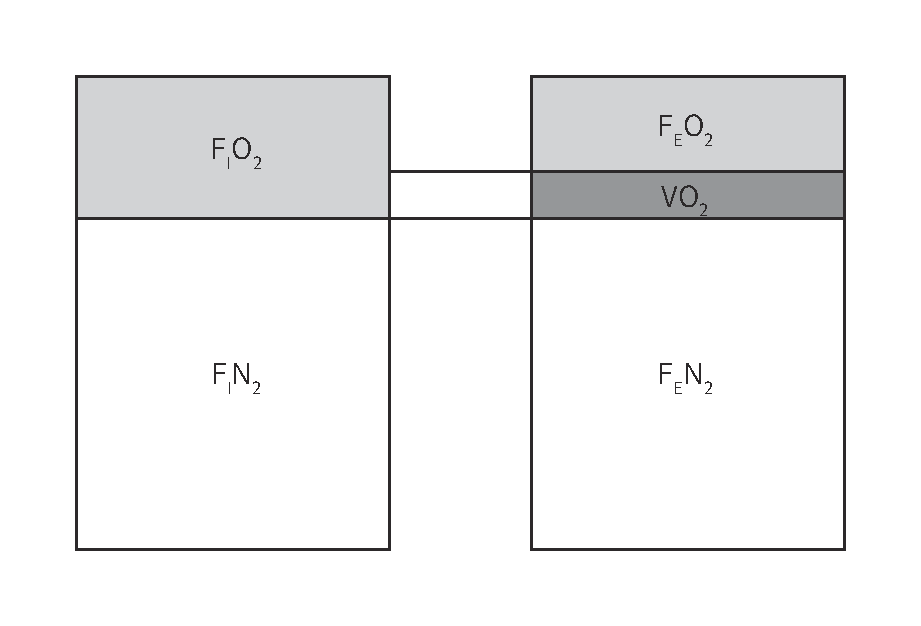
\includegraphics[width=8cm]{fig/vo2_measurement}
    \caption{VO_2測定の原理}
    \label{fig:vo2_measurement}
  \end{center}
\end{figure}

酸素摂取量\.{V}O_2は単位時間あたり(多くの場合1分間値が用いられる)に身体に取り入れられた酸素の量を表す値である.よって,吸気中酸素量\.{V}_IO_2と呼気中酸素量\.{V}_EO2の差が酸素摂取量となる.吸気中酸素量,呼気中酸素量は,それぞれ吸気中酸素濃度F_IO_2と呼気中酸素濃度F_EO_2を用いて式\ref{eq:vo2_principle}のように表せる.

\begin{equation}
  \label{eq:vo2_principle}
  \.{V}O_2 = (\.{V}_I \times F_IO_2) - (\.{V}_E \times F_EO_2)
\end{equation}

よって,酸素摂取量は吸気中酸素量と呼気中酸素量を測定することにより求められる.しかし,実際には呼気の分析のみで酸素摂取量を求めることができる.

\subsubsection{窒素補正}
\label{sec:n2}

呼気の分析のみで酸素摂取量を求めるためには,{\bf 窒素は代謝に使われないため,身体に吸収されない}という性質を利用する.この性質から,吸気中窒素濃度F_IN_2と呼気中窒素濃度F_EN_2を用いて式\ref{eq:vi_vefen2}が成り立つ.

\begin{equation}
  \label{eq:vi_vefen2}
  \.{V}_I \times F_IN_2 = V_E \times F_EN_2
\end{equation}

\.{V}_Iに関してまとめると,\.{V}_Iは式\ref{eq:vi_ve}のように表せる.

\begin{equation}
  \label{eq:vi_ve}
  \.{V}_I = \frac{\.{V}_E \times F_EN_2}{F_IN_2}
\end{equation}

これを式\ref{eq:vo2_principle}に代入すると次のようになる.

\begin{equation}
  \label{eq:vo2_ve}
  \.{V}O_2 = \frac{\.{V}_E \times F_EN_2}{F_IN_2} \times F_IO_2 - \.{V}_E \times F_EO_2
\end{equation}

式\ref{eq:vo2_ve}の右項から,\.{V}_Eを括り出すことで次の式が成り立つ.

\begin{equation}
  \label{eq:vo2_n2}
  \.{V}O_2 = \.{V}_E \times (\frac{F_EN_2}{F_IN_2} \times F_IO_2 - F_EO_2)
\end{equation}

\begin{equation}
  (酸素摂取量) = (呼気量) \times (酸素摂取量\%)
\end{equation}

つまり,式\ref{eq:vo2_n2}は,酸素摂取量は呼気量と酸素摂取率の積で表されることを示している.

式\ref{eq:vo2_n2}の右項の

\begin{equation}
  \frac{F_EN_2}{F_IN_2} \times F_IO_2
\end{equation}

の部分は,「窒素は代謝に使われないため,吸気と呼気中の窒素の量は変わらない」という特性を利用して,吸気中の酸素濃度を呼気量に相当した酸素濃度に換算していることを意味している.このような換算を窒素補正と呼ぶ\cite{calculate_vo2_resume}.

呼気中窒素濃度は呼気中酸素濃度と呼気中二酸化炭素濃度を100\%から引いた残りであるから,
式\ref{eq:vo2_n2}のF_EN_2はF_EO_2とF_ECO_2を用いて式\ref{eq:vo2_100_n2}のように表せる.

\begin{equation}
  \label{eq:vo2_100_n2}
  \.{V}O_2 = \.{V}_E \times (\frac{100 - F_EO_2 - F_ECO_2}{F_IN_2} \times F_IO_2 - F_EO_2)
\end{equation}

通常大気中において,吸気中窒素濃度F_IN_2は79.04\%,吸気中酸素濃度F_IO_2は20.93\%であるから,これらを代入して式\ref{eq:vo2_100_n2}は次のようになる.

\begin{equation}
  \label{eq:vo2_final}
  \.{V}O_2 = \.{V}_E \times (\frac{100 - F_EO_2 - F_ECO_2}{79.04} \times 20.93 - F_EO_2)
\end{equation}

式\ref{eq:vo2_final}から,呼気量V_Eと呼気中酸素濃度F_EO_2,呼気中二酸化炭素濃度F_ECO_2から酸素摂取量VO_2を求めることができる.

\subsection{二酸化炭素呼出量}

呼吸代謝において,身体の中で作り出される二酸化炭素の量を二酸化炭素呼出量と呼ぶ.二酸化炭素呼出量\.{V}CO_2(L/min)は単純に,STPD(\ref{eq:stpd})における換気量\.{V}_Eと呼気中二酸化炭素濃度を掛けて求めることができる.この式は式\ref{eq:vco2}のようになる.

\begin{equation}
  \label{eq:vco2}
  \.{V}CO_2 = \.{V}_{STPD} \times F_ECO_2
\end{equation}

\subsection{呼吸交換比}

呼吸交換比(RER,respiratory exchange ratio)は呼吸における酸素摂取量に対する二酸化炭素呼出量の比率を表す.すなわち,計算式は式\ref{eq:rer}のようになる.

\begin{equation}
  \label{eq:rer}
  RER = \frac{\.{V}CO_2}{\.{V}O_2}
\end{equation}

呼吸交換比は運動量が大きくなるほど大きくなり,この値によって,エネルギーが生成される際の化学反応から,体内でどのような割合で栄養素が燃焼しているかの目安とすることができる.

%\subsection{呼吸商}

\subsection{運動強度}

運動強度の指標として使われるMETs(メッツ)は,安静時と1とした時と比較して何倍の運動強度であるかということを表す値である.
この値において,安静時とは体重あたりの酸素摂取量\.{V}CO_2}(mL/kg/min)を用いて3.5mL/kg/minと定義されている.酸素摂取量を測定することで,運動中の酸素摂取量からMETs値をリアルタイムで計算することが可能である(式\ref{eq:mets}).

\begin{equation}
  \label{eq:mets}
  \.{METs} = \frac{\.{V}O_2}{3.5}
\end{equation}

\subsection{消費エネルギーの推定}

\subsubsection{直接法}

人体で消費されたエネルギーは熱となって放射される.その熱量を直接測るのが直接法である.例えば,直接法の測定機器であるAtwater-Benedict-Rosa calorimeterでは,測定室内の被験者が放射する熱を室内に張り巡らされた管を流れる水の温度から測定する.それに加え,室内で発生した水蒸気量呼気などの水蒸気の気化熱を測定するとともに,測定中の体温の変化も考慮して,被験者のエネルギー消費量を測定する\cite{tanaka_2006}.

このように装置が大掛かりで,活動内容も測定室内で行えるものに限られるため,現在でも使用は一部の実験施設などに限られている.

\subsubsection{間接法}

そこで,測定が容易な別の値から間接的に消費エネルギーを求める方法が考案されてきた.その中でも,心拍数を用いて消費エネルギーを推定する方法は,安静時心拍数と最大心拍数から運動強度を算出するカルボーネン法\cite{karvonen_1988}などが様々な心拍数を測定できるデバイスやサービスで利用されている.

しかし,心拍数は気温や体調による影響を受けやすいため,日によるばらつきが大きく,これを用いた消費エネルギーの推定は精度面で問題が残る.そこで,より正確に消費エネルギーを推定する方法として,呼気分析によって消費エネルギーを推定する方法がある.

\subsubsection{Weirの式}

人体がエネルギーを生み出す際の化学反応から消費エネルギーを推定することができる.食物から取り込んだ栄養素が酸素と反応し,二酸化炭素を産出する.この化学式を用いて,酸素摂取量と二酸化炭素摂取量,尿素窒素量が正確に得られれば,エネルギー消費量が1\%もしくはそれ以下の誤差で推定できる\cite{livesey_1988}.

例えば,よく利用されるWeir\cite{weir_1949}の式は式\ref{weir_urea_formula}の通りである.

\begin{equation}
  \label{weir_urea_formula}
  EE(kcal) = 3.941 \times 酸素摂取量 + 二酸化炭素産生量 - 2.17 \times 尿中窒素排出量
\end{equation}

このうち,尿素窒素排出量は摂取エネルギーに閉めるたんぱく質の割合によって決まる.この値は比較的安定しており,たんぱく質の占める割合を12.5\%と仮定するとWeirの式は式\ref{eq:weir_formula}のようになる.

\begin{equation}
  \label{eq:weir_formula}
  EE(kcal) = 3.9 \times 酸素摂取量 + 1.1 \times 二酸化炭素産生量
\end{equation}

尿中窒素排出量を使用しないWeirの式は,たんぱく質の占める割合が20\%を大きく超えるような極端に偏った食事や,激しい運動中に限定したりすることをしなければ,誤差の影響は1\%未満であり,酸素摂取量と二酸化炭素産出量のみでも十分に正確に測定することができるという\cite{tanaka_2006}.

\expandafter\ifx\csname ifdraft\endcsname\relax
  \end{document}
\fi
